\typeout{ ====================================================================}
\typeout{ this is file intro.tex, created at 16-Jun-2016               }
\typeout{ maintained by Gustavo Rabello dos Anjos                             }
\typeout{ e-mail: gustavo.rabello@gmail.com                                   }
\typeout{ ====================================================================}


\section{INTRODUÇÃO}

Escoamentos multifásicos são caracterizados quando há presença de mais
de uma fase no escoamento, onde entende-se por fase a região do espaço
delimitada por uma interface que a separa de outra fase. É importante
notar que um escoamento multifásico pode conter o mesmo tipo de
substância presente em fases distintas. Esse é o caso, por exemplo, de
água escoando em um radiador (trocador de calor) de automóvel. Nesse
caso encontra-se no mesmo sistema água no estado líquido, antes de
entrar em contato com o óleo aquecido do motor, e água em estado gasoso,
depois de absorver calor do óleo e o líquido trocar de fase. Este
escoamento multifásico é considerado de material único, porém de
múltiplas fases. Na tabela~\ref{table1} encontram-se exemplos de
misturas multifásicas, como a chuva que se caracteriza pelo escoamento
de gotas de água imersas em ar e também de escoamentos monofásicos com
vários materiais, que é o caso do escoamento de ar composto de diversos
gases em uma fase única homogênea.

\begin{center}
  \begin{tabular}{ccc}
    \hline
    material & fase única  & fases diferentes \\
    \hline
    único    & escoamento de água em dutos & líquido em ebulição \\
    variado  & mistura de gases do ar      & chuva (escoamento de água e ar)  \\
    \hline\\
  \end{tabular}
  \tabcaption{Exemplos de escoamentos multifásicos encontrados na
  natureza com diversos materiais e fases.}
  \label{table1}
\end{center}


\subsection{Abordagem Empírica ou Experimental}

Para iniciarmos a introdução às técnicas experimentais, passamos
pela definição de importantes parâametros utilizados na
caracterização do escoamentos bifásicos. A seguir, serão
identificados padrões encontrados frequentemente em escoamentos
multifásicos em canais verticais e horizontais. é importante notar
que a literatura disponível em escoamentos com mais de uma fase é
extenso e não se limita aos exemplos introdutórios apresentados
neste capítulo. Ao leitor que deseja aprofundar tais conceitos,
sugerimos \cite{collier1996}, \cite{whalley1987} e \cite{carey2007}.

\subsection{Título de vapor}

O título de vapor ($x$) é definido pela razão da vazão
mássica de vapor ($\dot{M}_G$) dividida pela vazão mássica total
($\dot{M}_G+\dot{M}_L$):

\begin{equation}
	x = \frac{\dot{M}_G}{\dot{M}_G+\dot{M}_L}
\end{equation}

Quando o escoamento é adiabático, ou seja não há transferência
de calor, se torna necessário a medida de vazão mássica para cada
fase, com isso o título de vapor é determinada para todo o tubo. Se
o tubo é aquecido e fluxos de massa são notados no sistema, o
título de vapor aumentará na direção do escoamento. No
entanto, para o caso de resfriamento do tubo e, consequentemente, a
condensação do vapor, o título de vapor diminuirá na direção do escoamento.

\subsection{Velocidades}

Em escoamentos multifásicos existem um grande número de velocidades
que podem ser definidas experimentalmente. Ainda, como os fluidos
estão em fases distintas, diferentes velocidades podem ser
encontradas, sugerindo também o uso de velocidade relativa como base
para caracterização da velocidade do escoamento. A seguir são
definidas algumas importantes velocidades encontradas na literatura.

\begin{itemize}
	\item Velocidade média verdadeira: é a velocidade em que cada fase
	se movimenta no escoamento.
	\item Velocidade superficial: também conhecida como fluxo
	volumétrico, é definida como a razão do fluxo de velocidade da fase
	considerada pela área transversal total do escoamento multifásico.
	\item Velocidade de deriva: razão da velocidade verdadeira média
	pela velocidade superficial total.
\end{itemize}

\subsection{Fluxo de massa}

O fluxo de massa ($G$) é definido como a vazão mássica total ($\dot{M}$)
divida pela área transversal do escoamento:

\begin{equation}
	G = \frac{\dot{M}}{A}
\end{equation}

\noindent onde a expressão acima representa a relação entre a velocidade
média do escoamento multiplicada pela densidade média. A unidade usual
de fluxo de massa é $[kg/m^2 s]$.

\subsection{Fração de vazios}

A fração de vazios $\epsilon$ é um dos parâmetros mais importantes para
caracterização de escoamentos multifásicos. Este também é de grande
importância para a determinação de outros parâmetros, tais como
viscosidade e densidade em escoamentos multifásicos, obtenção de
velocidade média relativa e, também, como ferramenta fundamental em
modelos de previsão de transição de padrões de escoamentos. 

Na literatura existem várias definições para especificação de fração de
volume (veja \cite{thome2008}). Aqui serão apresentadas as principais
definições de fração de vazios: local, cordal, transversal e
volumétrica. 

A fração de vazios local $\epsilon_{local}$ é tipicamente medida em um
ponto ou pequeno volume quando feita experimentalmente. é definida com
$\epsilon_{local} = 0$ quando líquido está presente ou $\epsilon_{local}
= 1$ quando vapor está presente. Tipicamente é realizada uma média
temporal local para determinção da fração de vapor, sendo definida pela
seguinte expressão:

\begin{equation}
	\epsilon_{local}(r,t) 
	= 
	\frac{1}{t} \int_t P_k(r,t) dt
\end{equation}

\noindent onde $P_k(r,t)$ é uma função indicadora da presença de vapor
no ponto em função do tempo $t$.

A fração de vazios cordal $\epsilon_{local}$ é tipicamente medida
através de um feixe radioativo brilhante que atravessa o tubo onde o
escoamento multifásico está localizado. Através da absorção de luz deste
feixe no outro lado do tubo, é possível medir o comprimento da fase
gasosa. A vazão de vazios cordal é então determinada por: 

\begin{equation}
	\epsilon_{cordal} = \frac{L_G}{L_G+L_L}
\end{equation}

\noindent onde $L_G$ é o comprimento de linha na fase gasosa e $L_L$ na
fase líquida.

A fração de vazios transversal $\epsilon_{trans}$, é medida a partir de
meios óticos ou através de medidas indiretas, tal como a capacitância
elétrica de uma fase líquida condutora. Esta fração é definida como:

\begin{equation}
	\epsilon_{trans} = \frac{A_G}{A_G+A_L}
\end{equation}

\noindent onde $A_G$ é a área ocupada da fase gasosa e $L_L$
da fase líquida.

A fração de vazios volumétrica $\epsilon_{vol}$ é medida geralmente
através de mecanismos de armadilha para os fluidos, onde por um instante
breve a amostra fica armazenada, possibilitando a medida da quantidade
de gás e líquido diretamente. Esta fração é então definida como:

\begin{equation}
	\epsilon_{vol} = \frac{V_G}{V_G+V_L}
\end{equation}

\noindent onde $V_G$ é o volume ocupado da fase gasosa e $L_L$ da fase
líquida.

\subsection{Escoamentos verticais}

Os padões de escoamentos para cima em tubos verticais é apresentado
esquematicamente na Fig.~(\ref{fig:vertical}). As diferenças básicas
observadas experimentalmente são descritas a seguir. é importante notar
que a utilização de cada padrão de escoamento depende da sua aplicação. 

\begin{figure}[h!]
	\begin{center}
		\subfloat[Bolhas]
		{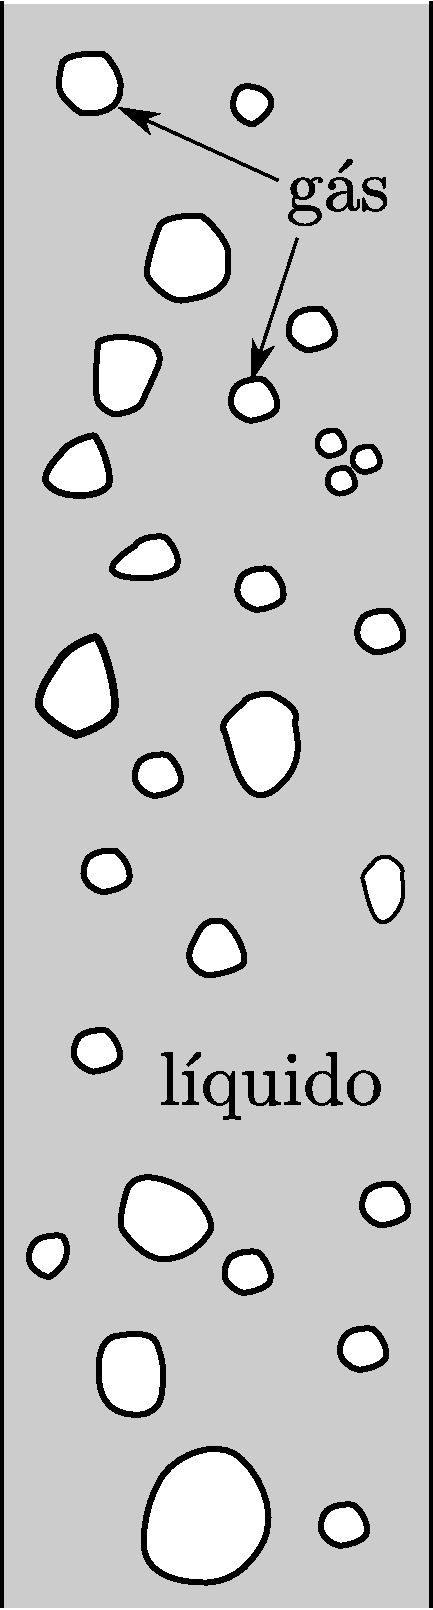
\includegraphics[angle=00, scale=0.3]{figs/v_bubbly.pdf}
		\hspace{0.8cm}}
		\subfloat[Golfada]
		{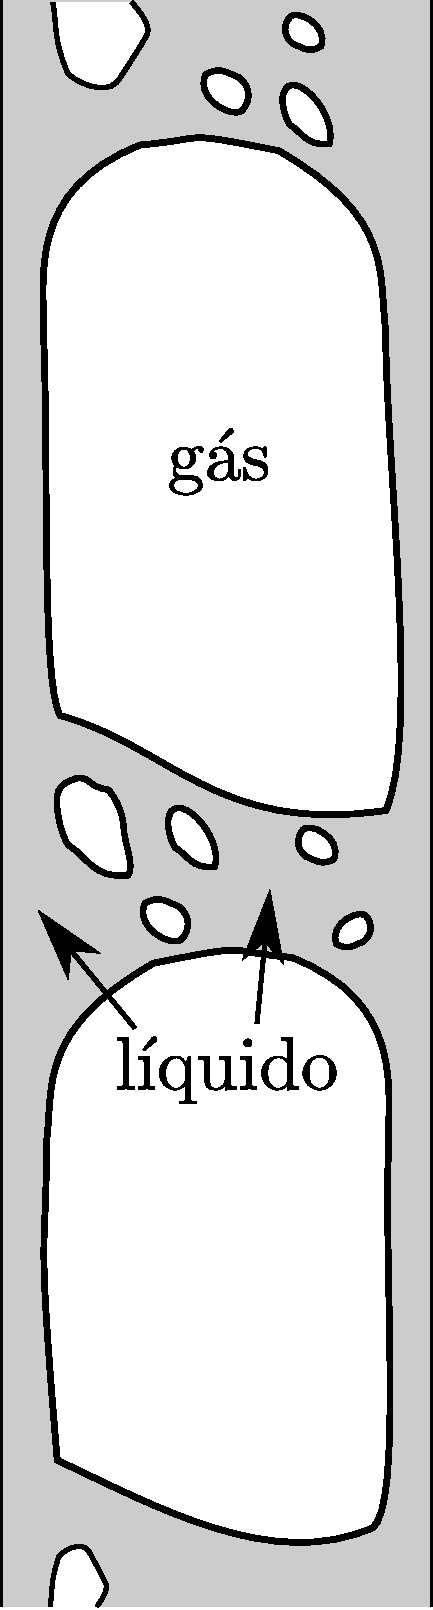
\includegraphics[angle=00, scale=0.3]{figs/v_slug.pdf}
		\hspace{0.8cm}}
		\subfloat[Batido]
		{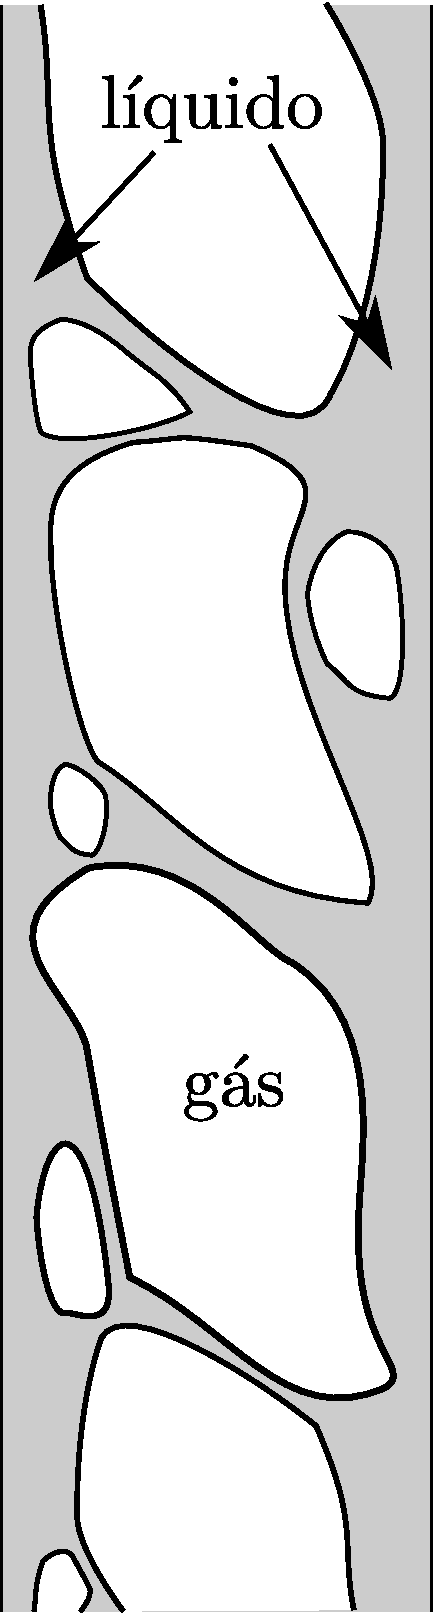
\includegraphics[angle=00, scale=0.3]{figs/v_churn.pdf}
		\hspace{0.8cm}}
		\subfloat[Pouco anular]
		{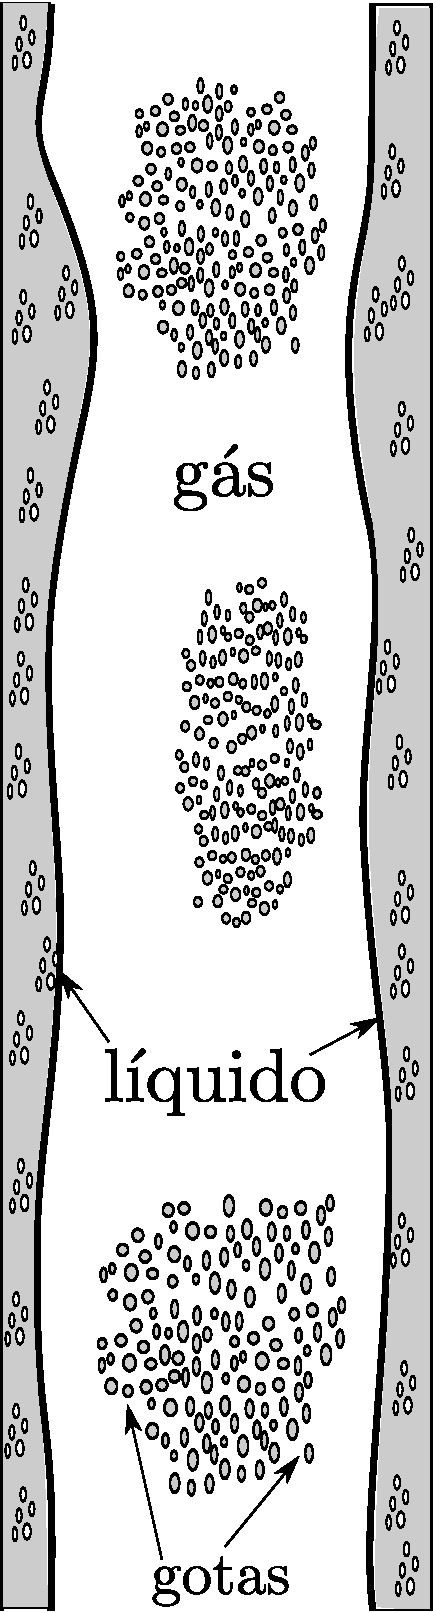
\includegraphics[angle=00, scale=0.3]{figs/v_wispy-annular.pdf}
		\hspace{0.8cm}}
		\subfloat[Anular]
		{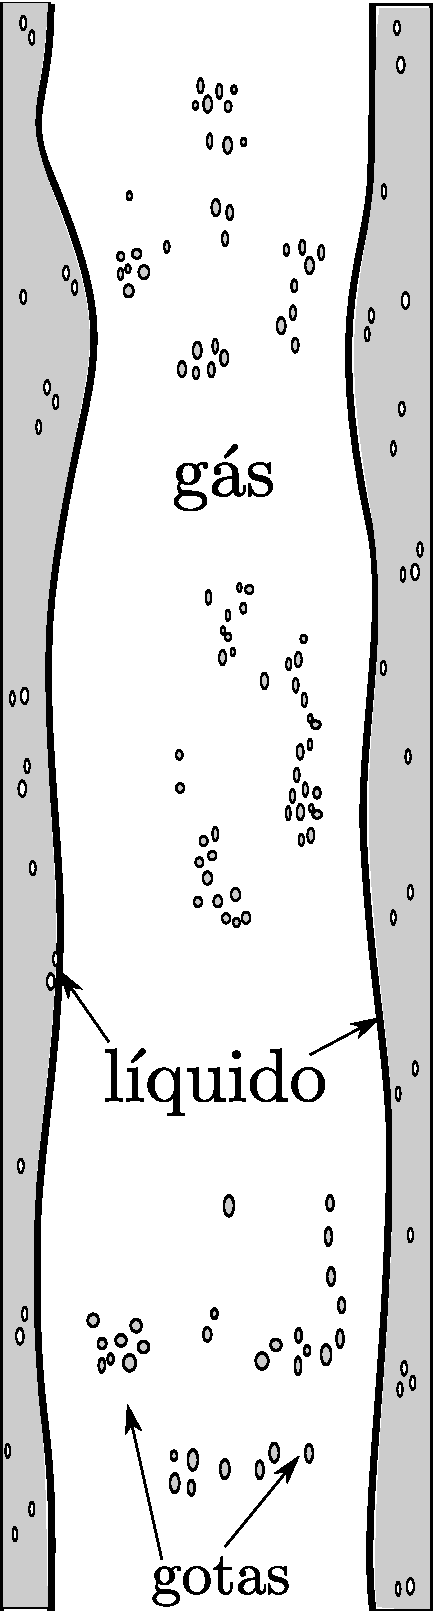
\includegraphics[angle=00, scale=0.3]{figs/v_annular.pdf}}
	\end{center}
	\caption[Escoamentos bifásicos em tubos verticais.]{Escoamentos
	bifásicos em tubos verticais. Em todos os casos o escoamento se faz
	de baixo para a cima. Os efeitos gravitacionais são uniformes ao
	longo do eixo horizontal, fazendo com que o escoamento apresente
	alguma estrutura simétrica.} \label{fig:vertical} 
\end{figure}

\begin{itemize}
	\item Bolhas dispersas: no escoamento em bolhas, o gás ou a fase
	vapor está distribuída na fase contínua líquida como um aglomerado
	de bolhas. Em uma situação extrema, estas bolhas podem apresentar
	formato esférico e de pequeno diâmetro ou apresentar formato de
	corpo alongado com a uma das extremidades arredondadas. Neste último
	estado, mesmo não apresentando tamanhos comparáveis ao diâmetro do
	tubo, o padrão das bolhas pode trazer alguma semelhança ao
	escoamento em golfadas.
	\item Golfadas: neste tipo de escoamento, as bolhas apresentam
	aproximadamente o mesmo diâmetro do tubo, com isso os efeitos de
	parede são mais evidentes. O nariz da bolha tem um formato
	característico arredondado devido à pressão e ao escoamento,
	enquanto que as laterais são separadas por um filme líquido que vai
	suavemente diminuindo até chegar à parte de trás da bolha. O termo
	golfadas representa o líquido que separa sucessivas bolhas de gás ou
	vapor. Dependendo do escoamento, pequenas bolhas podem ou não estar
	presentes entre as bolhas principais.
	\item Batido: a interface de largas bolhas de gás ou vapor se
	quebra, formando o escoamento do tipo golfadas em uma distribuição
	caótica. Nele, a fase líquida é empurrada em direção às paredes do
	canal. Este escoamento também é conhecido como semi-anular ou
	golfada-anular, devido ao carárter transitório deste padrão.
	\item Pouco anular: o filme líquido apresenta grande espessura nas
	paredes do tubo com uma considerável quantidade de líquido arrastada
	para dentro do núcleo de gás ou vapor. Este tipo de padrão de
	escoamento foi primeiramente identificado pelo trabalho de
	\cite{hewitt1970}. Em um padrão geral, muitas bolhas são encontradas
	no filme líquido próximo às parades do tubo, enquanto que grandes
	gotas são arrastadas dentro do núcleo de gás ou vapor. Este padrão
	de escoamento é encontrado em grandes vazões mássicas e, devido á
	grande quantidade de bolhas no filme líquido, este escoamento pode
	ser confundido com o escoamento em bolhas. 
	\item anular: um filme líquido é formado próximo às paredes do tubo
	devido ao aparecimento de um núclo contínuo de gás ou vapor no meio
	do tubo. O aparecimento de ondas pode ser notado na superfície do
	filme. Devido a sucessiva quebra destas ondas, pode haver a formação
	de gotas no núcleo de gás ou vapor. Diferentemente do escoamento do
	tipo pouco anular, as gotas estão separadas ao invés de aglomeradas.
\end{itemize}

\subsection{Escoamentos horizontais}

Os padrões de escoamento comumente encontrados em tubulações horizontais
e inclinados são complexos devido à sua natureza não simétrica causada
pelo influência do campo gravitacional. Entretanto são bem considerados
até hoje os padrões multifásicos sugeridos por \cite{alves1954} e
apresentados de forma esquemática na Fig.~(\ref{fig:horizontal}). 

\begin{figure}[h!]
	\begin{center}
		\subfloat[Bolhas dispersas]
		{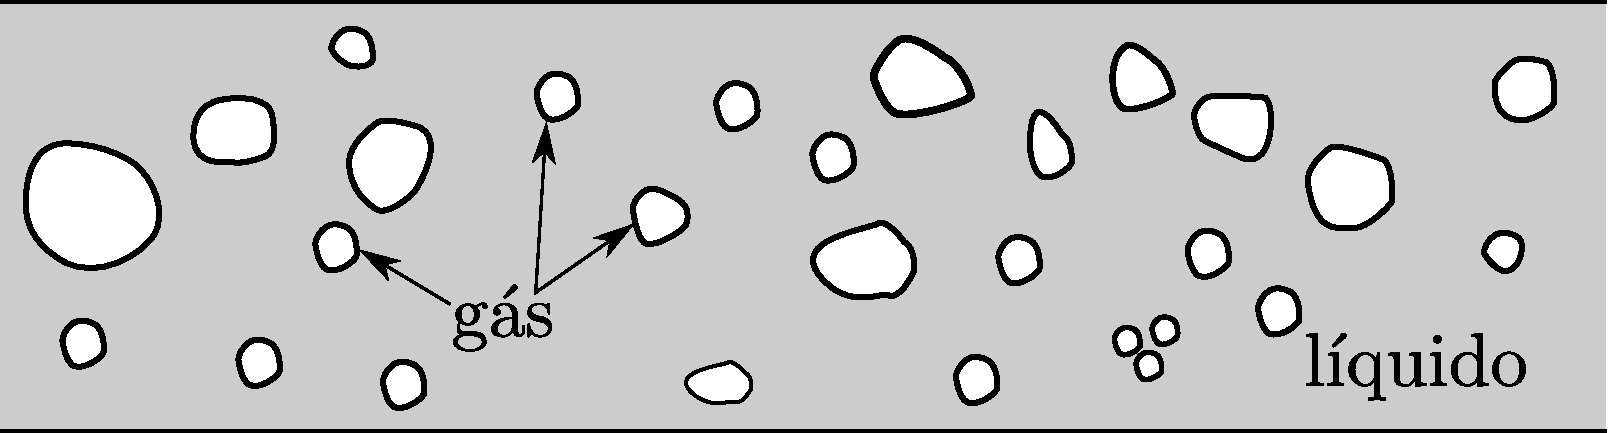
\includegraphics[angle=00, scale=0.265]{figs/h_bubbly.pdf}
 		\hspace{0.2cm}}
		\subfloat[Bolhas]
		{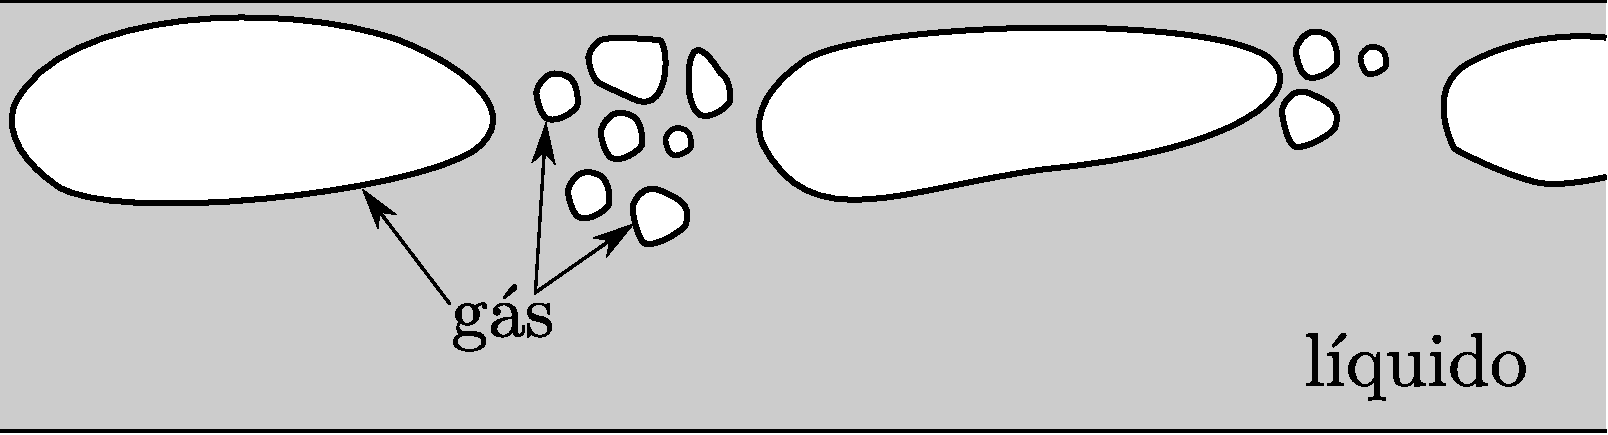
\includegraphics[angle=00, scale=0.265]{figs/h_plug.pdf}}\\
		\subfloat[Golfadas]
		{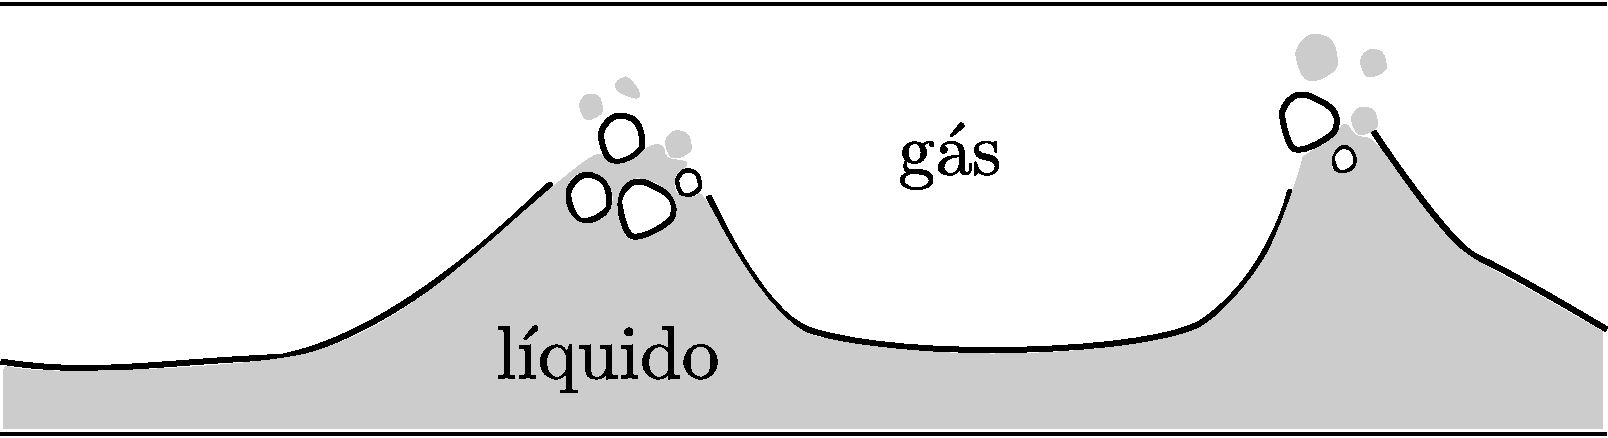
\includegraphics[angle=00, scale=0.265]{figs/h_slug.pdf}
 		\hspace{0.2cm}}
		\subfloat[Estratificado]
		{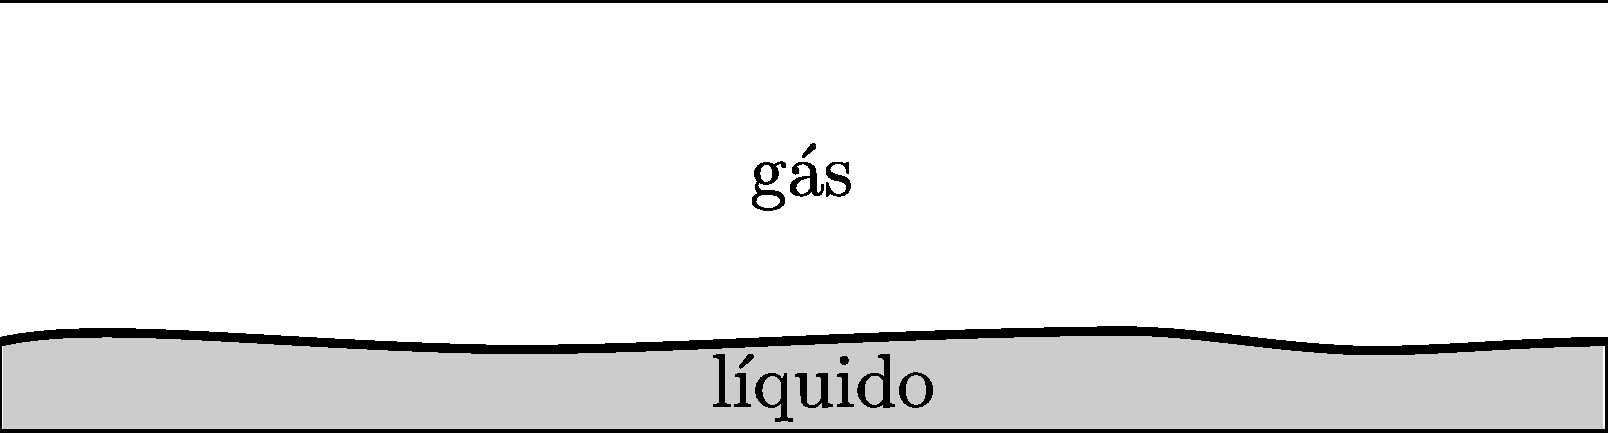
\includegraphics[angle=00, scale=0.265]{figs/h_stratified.pdf}}\\
		\subfloat[Estratificado ondulado]
		{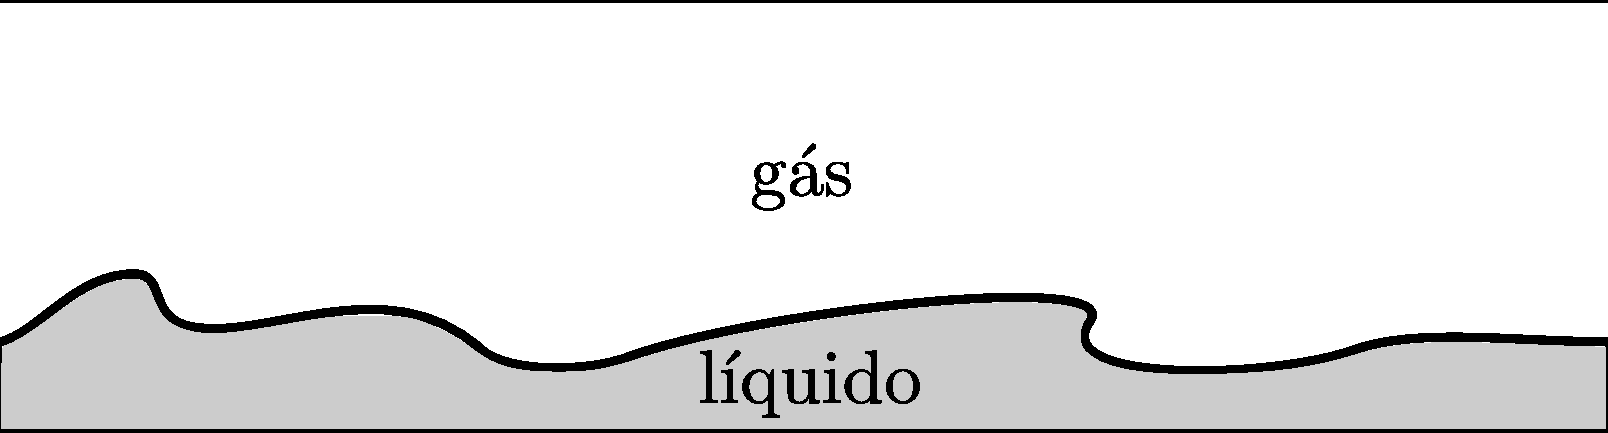
\includegraphics[angle=00, scale=0.265]{figs/h_wavy.pdf}
 		\hspace{0.2cm}}
		\subfloat[Anular]
		{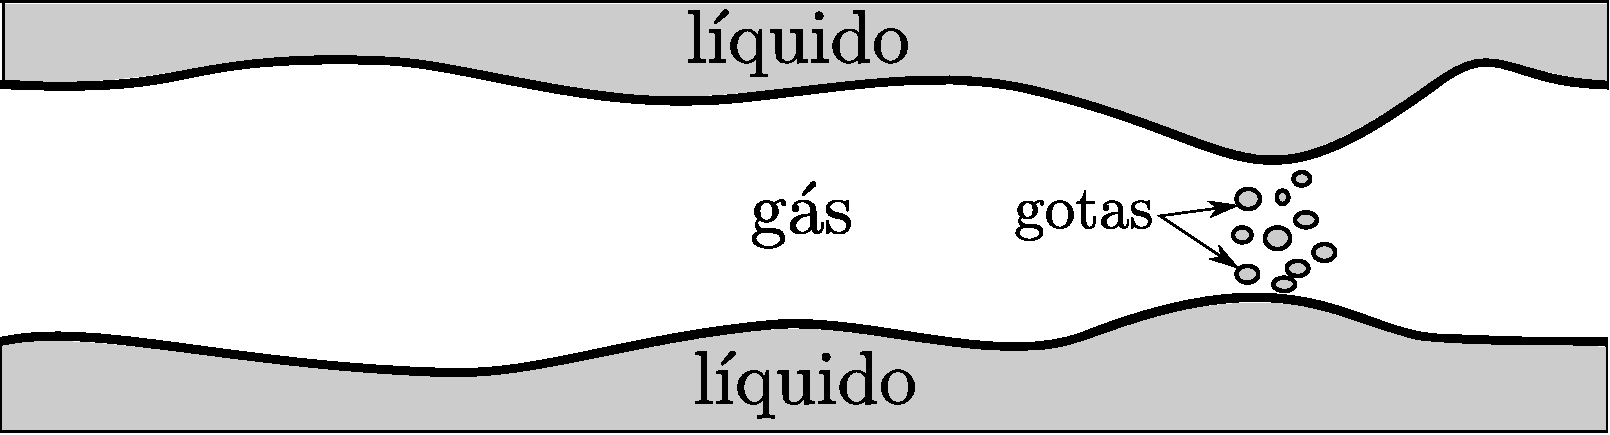
\includegraphics[angle=00, scale=0.265]{figs/h_annular.pdf}}
	\end{center}
	\caption[Escoamentos bifásicos em tubos horizontais.]{Escoamentos
	bifásicos em tubos horizontais. Em todos os casos o escoamento se
	faz da esquerda para a direta. Dependendo da velocidade de entrada
	das fases, um padrão pode ser identificado. Como pode ser verificado
	pela posição das bolhas, a gravidade exerce uma influência imediata
	nas fases, uma vez que o fluido menos denso tende a se movimentar na
	parte de cima do tubo.}
  \label{fig:horizontal} 
\end{figure}

\begin{itemize}
	\item Bolhas dispersas: este escoamento é similar ao apresentado
	anteriormente para escoamento vertical, com a diferença que as
	bolhas de gás ou vapor tendem a se movimentar na metade superior do
	tubo. Fato justificado pela menor densidade da bolha comparada ao
	líquido. Em uma velocidade moderada de ambas as fases presente no
	escoamento, a distribuição de bolhas é uniforme ao longo do tubo,
	enquanto que para velocidades mais elevadas o padrão de escoamento
	se assemelha ao pouco anular.
	\item Bolhas: escoamento similar ao do tipo golfadas em tubos
	verticais. Como no caso de bolhas dispersas, a bolhas de gás ou
	vapor tendem a atravessar o tubo na metade superior, devido ao campo
	gravitacional.
	\item Estratificado: escoamento separado por uma interface suave,
	onde geralmente é encontrado em baixas velocidades das fases líquida
	e gasosa.
	\item Estratificado ondulado: as ondas são formadas quando a
	velocidade na fase gasosa é aumentada. Estas ondas se movimentam na
	direcão do escoamento.  
	\item Golfada: com o aumento da velocidade da fase de vapor, a
	amplitude das ondas também aumenta, se aproximando da parede do
	tubo. A parte superior do tubo atrás da onda é molhada por um filme
	líquido que é drenado para o meio da fase líquido.
	\item Anular: a vazão da fase gasosa é tão alta que é capaz de
	sustentar a fase líquida próxima à parede do tubo, originando um
	núcleo de gás ou vapor. Em sua seção transversal, o líquido pode não
	ser contínuo ao redor de toda a circunferência, porém será mais
	espesso na base do tubo.
\end{itemize}

\subsection{Mapa de padrões de escoamentos}
Os mapas de padrões de escoamento são utilizados para a identificação do
tipo de escoamento (golfadas, anular, estratificado etc.) através de
parâmetros conhecidos como vazão mássica, fração de vazios, qualidade de
vapor etc. Estes mapas existem para diferentes tipos de fluidos,
dimensão de tubos, graus de mistura e muitos outros. Basicamente, eles
podem ser divididos em duas classes: adiabáticos e diabáticos. O
primeiro é usualmente utilizado para escoamentos do tipo ar/água,
enquanto o segundo pode ser encontrado em refrigerantes em evaporação. 

Os mapas de padrões são representados como áreas em gráficos, em função
das velocidades superficiais ou qualquer outro parâmetro geral que
contenha tal definição. É importante notar que o padrão de escoamento é
também influenciado por outros tipos de parâmetros, porém sua descricão
é feita através de gráficos bi-dimensionais. Na literatura, muitos mapas
podem ser encontrados para diferentes fluidos e em diferentes condições.
O leitor interessado poderá consultar algumas referências clássicas como
(\cite{collier1996}, \cite{whalley1987} e \cite{thome2008}).

A Fig.~(\ref{fig:map}a) representa um mapa de padrões de escoamento para
ar/água, em condições de pressão atmosférica, para canais verticais
baseado em (\cite{hewitt1969}). Neste mapa pode-se observar que cada
padrão de escoamento ocupa uma área no gráfico e as linhas tracejadas
delimitam a transicão. Como pode-se observar também, estas mesmas linhas
não ocupam todo o limite do gráfico, o que sugere a falta de dados
experimentais para descrever as transições em toda a escala. É
importante notar que estes mapas devem ser observados não mais do que um
guia grosseiro de padrões de escoamentos, pois os fluxos de quantidade
de movimento por si só não são capazes de representar com exatidão a
influência das propriedades físicas do fluido nem o diâmetro do tubo.

A Fig.~(\ref{fig:map}b) descreve um outro mapa de padrões, porém para
escoamento horizontal baseado em (\cite{baker1954}). Este mapa é
largamente utilizado na indústria petroquímica. No mapa pode-se
identificar os padrões de escoamento em diferentes velocidades mássicas
superficiais de líquido $G_L$ e de gás $G_G$. 

\begin{figure}[ht!]
	\subfloat[]
	{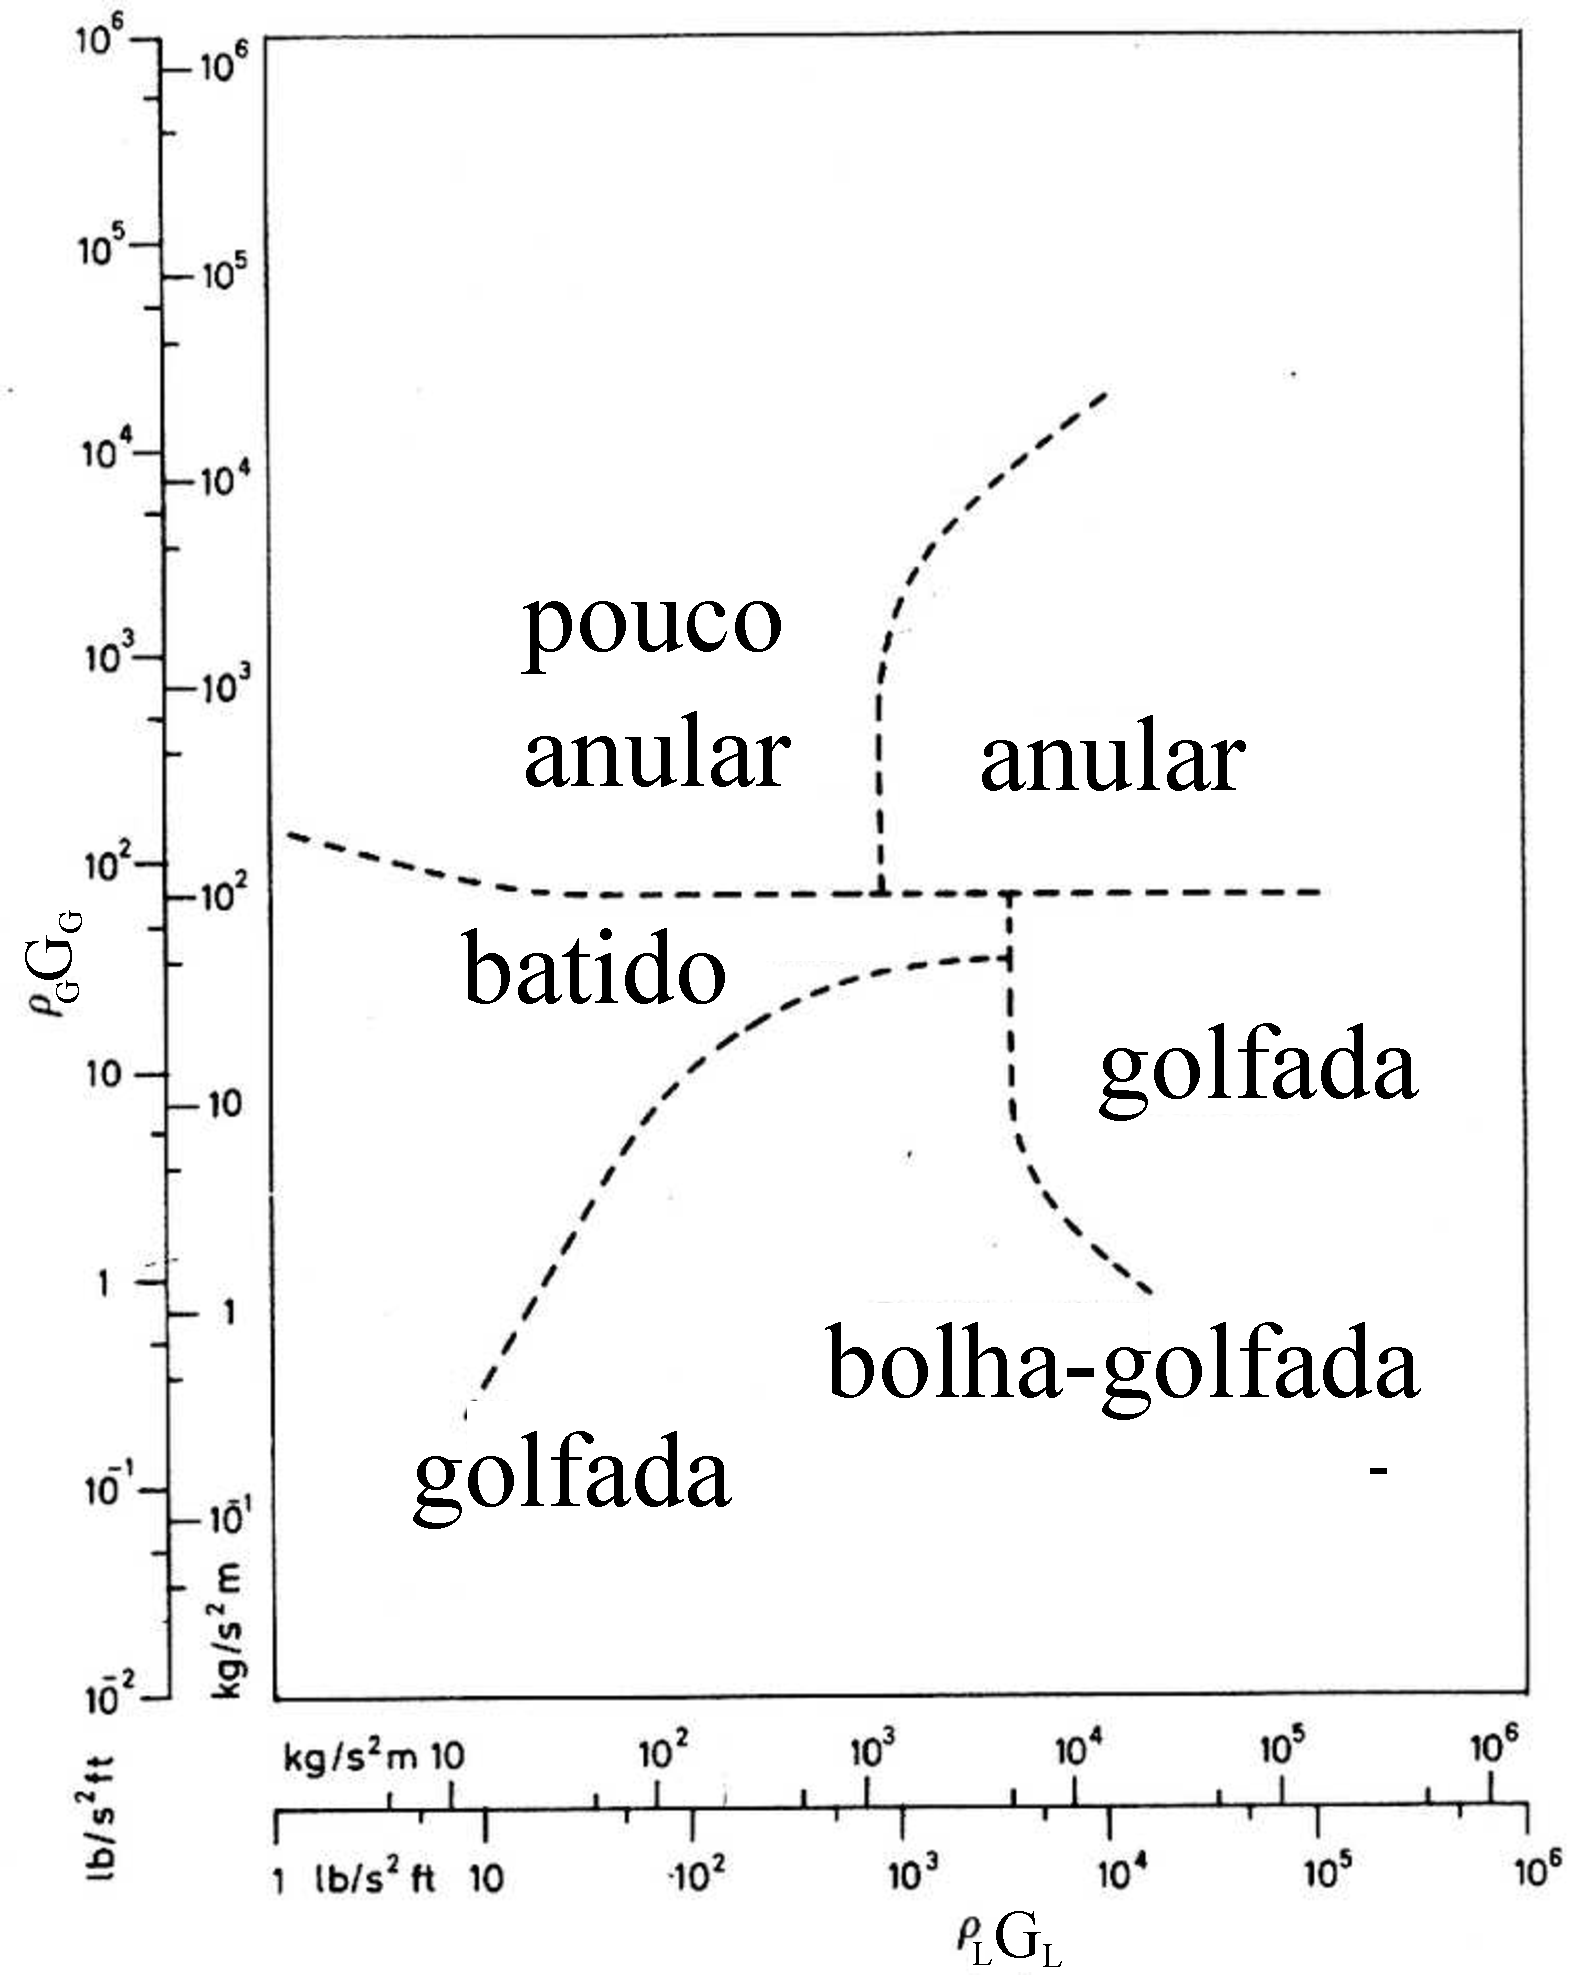
\includegraphics[scale=0.27,angle=-0.5]{figs/hewitt1969.pdf}}
	\hspace{0.2cm}
	\subfloat[]
	{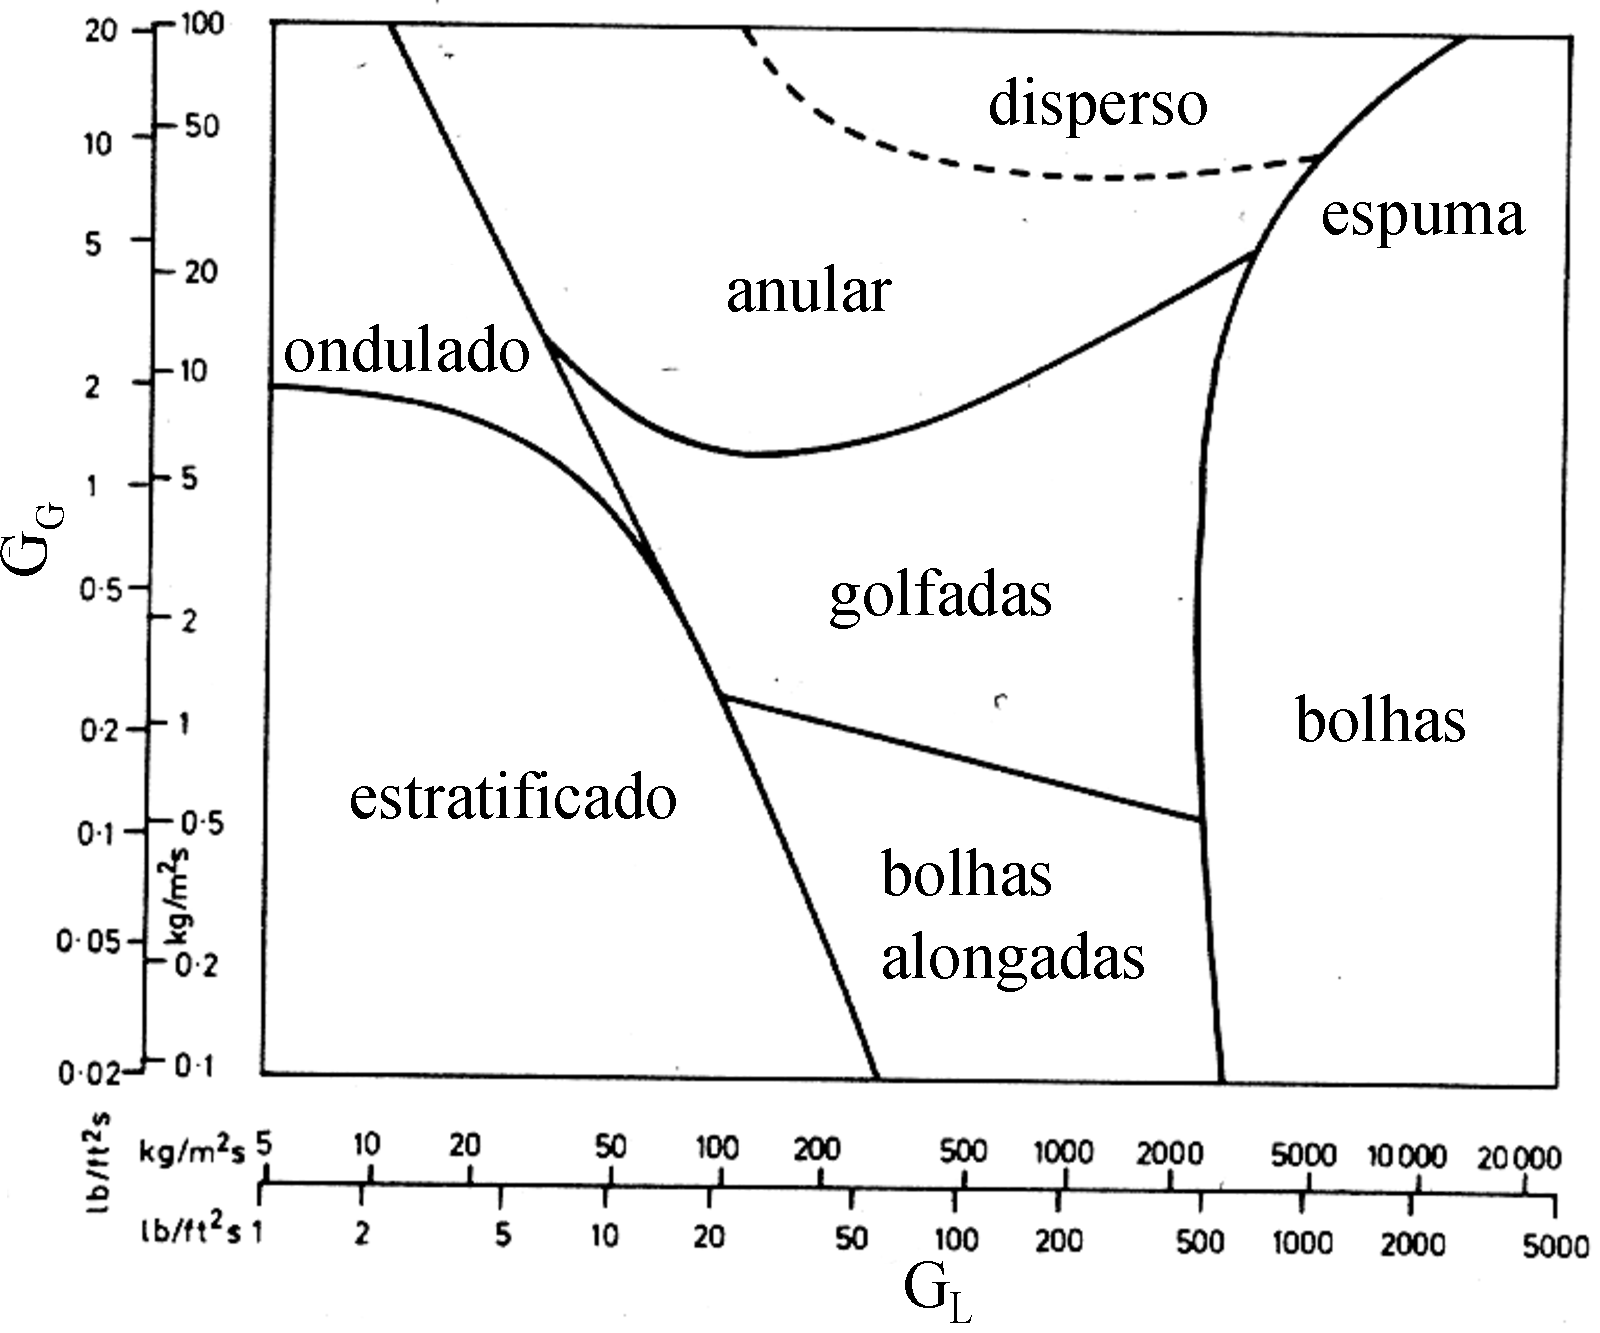
\includegraphics[scale=0.27,angle=1]{figs/baker1954.pdf}}
	\caption[Mapas de padrões de escoamento bifásico.]{Mapas de padrões
	de escoamento bifásico representado por fluxo de massa $G$ de
	líquido $G_L$ e de gás $G_G$. As linhas contínuas e tracejadas
	representam a transição dos padrões de escoamento. (a) Escoamento
	vertical para ar/água baseado em (\cite{hewitt1969}). (b) Escoamento
	horizontal para ar/água baseado em (\cite{baker1954}).}
	\label{fig:map} 
\end{figure}


\subsection{Perda de carga}
\subsubsection{Método homogêneio}
\subsubsection{Método de separação}
\subsubsection{Perda de carga em conjunto de tubos}
\subsubsection{Recomendações}

\subsection{Mudança de fase}
\subsubsection{Condensação}
\subsubsection{Formas de vaporização}
\subsubsection{Ebulição}


\typeout{ ****************** End of file intro.tex ****************** }

